\documentclass[a4paper]{article}
\usepackage[warn]{mathtext}
\usepackage{graphicx} % Required for inserting images
\usepackage{wrapfig}
\usepackage{enumitem}
\usepackage[center]{caption}
\usepackage[english, russian]{babel}
\usepackage{amsmath}
\usepackage{geometry}
\setcounter{totalnumber}{5}

\geometry{verbose, a4paper, tmargin=2cm, bmargin=2cm, lmargin=2.0cm, rmargin=2.0cm}

\begin{document}

\begin{titlepage}
	\centering
	{\scshape\Large МОСКОВСКИЙ ФИЗИКО-ТЕХНИЧЕСКИЙ ИНСТИТУТ \\
	(НАЦИОНАЛЬНЫЙ ИССЛЕДОВАТЕЛЬСКИЙ УНИВЕРСИТЕТ)\\ % название ВУЗа большим шрифтом
    Физтех-школа аэрокосмических технологий}
	
	\vspace{4cm} % отступ 4 см по вертикали
	{\LARGE Отчет о выполнении лабораторной работы 1.4.8}
	\vspace{1cm} % ещё 1 см
	
{\huge\bf Измерение модуля Юнга \\ методом акустического резонанса}
	
	\vspace{1cm} % ещё 1 см
	\vfill % заполнение по вертикали пустотой (LaTeX сам решит, сколько здесь отступить)
	
    \begin{flushright} % Этот текст будет с правого края страницы
	   {\LARGE Губарев Никита, Б03-502}
    \end{flushright}
    \vfill 
	\today % Дата сборки документа
\end{titlepage}
\tableofcontents 
 \section{Аннотация}
Цель работы: исследование явления акустического резонанса в тонком стержне; измерение скорости распространения продольных звуковых колебаний в тонких стержнях из различных материалов и различных размеров; измерение модулей Юнга различных материалов.

\section{Теоретические сведения}

Основной характеристикой упругих свойств твёрдого тела является его модуль Юнга $E$. Согласно закону Гука, если к элементу среды приложено некоторое механическое напряжение $\sigma$, действующее вдоль некоторой оси $x$ (напряжения по другим осям при этом отсутствуют), то в этом элементе возникнет относительная деформация вдоль этой же оси $E = \Delta x/x_0$. \vspace{0.2 cm} \\
Если с помощью кратковременного воздействия в некотором элементе твёрдого тела создать малую деформацию, она будет далее распространяться в среде в форме акустической волны. Волны, распространяющиеся вдоль оси, по которой происходит деформация, называются продольными. Скорость $u$ распространения такой волны в простейшем случае длинного тонкого стержня определяется соотношением
\begin{equation}
u = \sqrt{\frac{E}{\rho}},
\end{equation}
где $\rho$ -- плотность среды.  \vspace{0.2 cm} \\
В общем случае звуковые волны в твёрдых телах могут быть не только продольными, но и поперечными (деформация сдвига перпендикулярна распространению волны), однако в данной работе будет исследован наиболее простой случай упругих волн, распространяющихся в длинных тонких стержнях. Если длины волны $\lambda$ и стержня $L$ много больше его радиуса $R$, то такая волна может свободно распространяться лишь вдоль стержня, и его упругие свойства описываются только модулем Юнга. \vspace{0.2 cm} \\ 
Акустическая волна, распространяющаяся в стержне конечной длины $L$, отражается от торцов стержня. Если при этом на длине стержня укладывается целое число полуволн, то отражённые волны будут складываться в фазе с падающими, что приведёт к резкому усилению амплитуды их колебаний и возникновению акустического резонанса в стержне. Измеряя соответствующие резонансные частоты, можно определить скорость звуковой волны в стержне и, таким образом, измерить модуль Юнга его материала. \vspace{-0.2 cm} \\
Скорость u определяется как:
\begin{equation}
u = 2L\frac{f_n}{n},
\end{equation} 
где $n$ -- номер гармоники. \vspace{0.2 cm} \\
Согласно теории, зависимость $f_n(n)$ линейна, и для всех резонансных частот отношение $\frac{f_n}{n}$ постоянно. Однако, если в идеальном случае резонанс достигался бы при строгом совпадении частот $f = f_n$, в реальности возбуждение стоячей волны возможно при относительно малом отклонении частоты от резонансной. Амплитуда как функция частоты $A(f)$ имеет резкий максимум при $f = f_n$. При этом ширина резонансного максимума $\Delta f$ определяется добротностью $Q$ колебательной системы:
\begin{equation}
\Delta f \approx \frac{f_\text{рез}}{Q}
\end{equation}
Именно конечная ширина резонанса $\Delta f$ определяет в основном погрешность измерения частоты.

\section{Методика измерений}
\begin{enumerate}
\item Осуществить предварительную настройку
\item Раздвинуть датчики и поместить между ними исследуемый стержень
на подставку
\item Разместить электромагниты напротив торцов стержня так, чтобы
торцы стержня совпали с центрами датчиков, а зазор между полюсами электромагнита и торцевой поверхностью стержней составлял 1–3 мм. Плоскость магнитов должна быть строго перпендикулярна оси стержня.
\item Предварительно определить диапазон частот генератора, в котором
целесообразно искать резонансы. Для этого оценить частоту первого резо-
нанса по формуле $f_1=\frac{u}{2L}$, воспользовавшись табличным значением скорости продольных волн в тонком медном стержне: $u\approx 3,7*10^3 м/с$
\item Медленно перестраивая звуковой генератор вблизи расчетной частоты $f_1$ найти первый резонанс, наблюдая за амплитудой колебаний на
экране осциллографа. При приближении к резонансу амплитуда сигнала с
регистрирующего датчика (канал CH2) резко возрастает, а амплитуда опорного сигнала (канал CH1) не меняется. Для увеличения сигнала колебаний
стержня нужно очень осторожно придвигать датчики к торцам стержня, не
допуская прилипания стержня к датчикам
\item Определить значение первой резонансной частоты $f_1$ по индикатору
частотомера. Для экспериментальной оценки погрешности измерения резонансной частоты повторите измерение несколько раз
\item Получить резонансы на частотах, соответствующих следующим
(кратным) гармоникам. Для этого, плавно перестраивая генератор, добейтесь резонанса вблизи частот $f_n\approx nf_1$, где n=2,3.... Постарайтесь измерить резонансные частоты с как можно большим n. Запишите измеренные
значения частот
\item Определитm плотность $\rho$ материала стержня. Для этого взвесьте и измерьте штангенциркулем линейные размеры небольшого образца цилиндрической формы, изготовленного из исследуемого материала
\item Определитm среднее значение диаметра исследуемого стержня
$d=2R$, измерив его штангенциркулем в нескольких местах. Проверьте
справедливость приближения «тонкий стержень»: $R/ \lambda << 1$
\item Повторитm опыты п. 2–10 со стержнями из других материалов той же длины
\item Для стержня из дюраля провести дополнительный опыт: перестраивая генератор, добиться возбуждения первой гармоники $f_1$ резонансных колебаний в стержне при «половинной» частоте генератора $f=\frac{f_1}{2}$. Пронаблюдать на экране осциллографа фигуру Лиссажу (в режиме работы «X–Y») и зарисовать её. Постараться объяснить явление.
\item Определите добротность стержня как колебательной системы, измерив амплитудно-частотную характеристику одного из стержней $A(f-f_1)$ вблизи первого резонанса.
Ширина максимума функции $A(f-f_n)$ связана с добротностью $Q$ стержня как колебательной системы: если $\Delta f$— ширина амплитудно-частотной характеристики на уровне $A=\frac{A_{max}}{\sqrt{2}}$, то $Q=\frac{f_n}{\Delta f}$.
\item Повторить измерения п. 4–10, используя стержень меньшей длины и диаметра
\item Для каждого из исследованных стержней построить по результатам
измерений п. 2–10 графики зависимости частоты $f(n)$ от номера гармоники
n (по возможности разместите зависимости на одном графике). Убедиться
в том, что зависимость является линейной, проходящей через начало координат
\item Построить наилучшие прямые по экспериментальным точкам и
определите соответствующие значения скорости звука $u$ (если точек на графике недостаточно, определите $u$ по среднему значению отношения $f_n/n$).
\item Определить модули Юнга $E$ исследуемых материалов. Оценить
погрешности результатов. Сравнить результаты с табличными данными
\item Проделать расчёты п. 14–16 по результатам измерений на стержнях меньшей длины и меньшего диаметра (п. 13). Сравнить с результатами, полученными на длинных стержнях.
\end{enumerate}

\section{Результаты измерений и обработка данных}
\subsection{Добротность стержней}
Исследовалась добротность дюралюминиевого стержня, по следующим точкам:
\begin{table}[!ht]
	\centering
	\begin{tabular}{|c|c|}
		\hline
		Частота, КГц & Интенсивность, о.е. \\ \hline
		4,23624 & 1 \\ \hline
		4,2354 & 0,8 \\ \hline
		4,23477 & 0,6 \\ \hline
		4,23365 & 0,4 \\ \hline
		4,23073 & 0,2 \\ \hline
		4,2356 & 0,92 \\ \hline
		4,23501 & 0,72 \\ \hline
		4,23425 & 0,52 \\ \hline
		4,23678 & 0,8 \\ \hline
		4,23754 & 0,6 \\ \hline
		4,23858 & 0,4 \\ \hline
		4,24136 & 0,2 \\ \hline
		4,23633 & 0,92 \\ \hline
		4,23691 & 0,72 \\ \hline
		4,2377 & 0,52 \\ \hline
	\end{tabular}
\end{table}
Построив график нормального распределения (Приложение 1), можно найти добротность:
$f_1 = 4236.2 Гц$, $\Delta f = 2.3 Гц$. Таким образом, добротность дюралюминиевого стержня равна 1842.

\subsection{Измерение скорости $u$} 
Были проведены измерения со стандартными стержнями и одним укороченным и более тонким медным ($l_m=527\pm1 мм, r_m=5.00\pm0.05 мм$)
\begin{table}[h]
\caption{Частоты резонанса для стержней различных материалов} 
\centering
\begin{tabular}{|c|c|c|c|c|c|c|c|c|}
\hline
& 1 & 2 & 3 & 4 & 5 \\
\hline
$f_\text{меди},$ кГц & 3.247 & 6.510 & 9.747 & 12.987 & 16.223 \\
\hline
$f_\text{стали},$ кГц & 4.125 & 8.262 & 12.381 & 16.512 & 20.636 \\
\hline
$f_\text{дюрали},$ кГц & 4.236 & 8.476 & 12.710 & 16.945 & 21.172\\
\hline
$f_\text{меди мал},$ кГц & 3.805 & 7.611 & 11.413 & 15.215 & 19.013 \\
\hline
\end{tabular}
\end{table}

Т. к. зависимость $f_n$ от $n$ линейная, по методу наименьших квадратов (Приложение 2) \newline ($L=600.0\pm 0.5 мм$):

\begin{table}[!h]
\caption{Скорости распространения волн} 
\centering
\begin{tabular}{|c|c|c|c|c|c|c|c|c|c|c|}
\hline
& $k $, Гц & $\sigma_k$, Гц & $u$, м/с & $\sigma_u$, м/с \\
\hline
Медь & 3243 & 9 & 3892 & 18 \\
\hline
Сталь & 4127 & 6 & 4952 & 11 \\
\hline
Дюраль & 4234 & 5 & 5081 & 10\\
\hline
Медь мал& 3805 & 3 & 4010 & 10 \\
\hline
\end{tabular}
\end{table} 

\subsection{Измерение плотности стержней}

\[
\begin{gathered}
	\rho = \frac{m}{\pi R^2 \cdot L}; 
\end{gathered}
\]

\begin{table}[!h]
	\caption{Характеристики различных материалов} 
	\centering
	\begin{tabular}{|c|c|c|c|c|c|c|c|c|c|c|}
		\hline
		& L, мм & R, мм & m, г & $\rho$, кг/м$^3$ & $\sigma_{\rho}$, кг/м$^2$\\
		\hline
		Медь & 40.55 $\pm 0.05$ & 6.00 $\pm 0.05$& 40.335 $\pm 0.001$& 8795 & 8\\
		\hline
		Сталь & 41.10 $\pm 0.05$& 5.95 $\pm 0.05$& 36.928 $\pm 0.001$& 7997 & 7\\
		\hline
		Дюраль & 41.35 $\pm 0.05$& 6.15 $\pm 0.05$& 13.242 $\pm 0.001$& 2685 & 3\\
		\hline
	\end{tabular}
\end{table} 
\newpage
\subsection{Вычисление модуля Юнга}
Из формулы (1):
\[
\begin{gathered}
	E = \rho \cdot u^2; \text{ }
\end{gathered}
\]
$E_\text{меди} = 133 \pm 1$ ГПа; $E_\text{стали} = 196 \pm 1$ ГПа; $E_\text{дюрали} = 69.3 \pm 0.4$ ГПа; $E_\text{меди} = 141.4 \pm 0.8$ ГПа.
\subsection{Эксперимент с половиной резонансной частоты в дюралюминиевом стержне}
Выставив половину резонансной частоты для дюралюминиевого стержня можно наблюдать на осциллографе фигуру Лиссажу (приложение 3) с характерным отношением частот 1:2, это можно объяснить тем, что в таком случае на концах стержня волна отражается в симметричной относительно изначальной оси стержня фазе, резонанс не нарушается, но отношение к опорной частоте становится 2:1. 
\section{Выводы}
В результате работы была вычислена добротность дюралюминиевого стержня, измерены резонансные частоты, скорости распространения звуковой волны в стержнях, их плотности и модули Юнга. Для меди были проведены эксперименты с двумя разными стержнями:\newline
$Q_{дюр} = 1842$\newline
\begin{table}[!h]
	\caption{Скорости распространения волн} 
	\centering
	\begin{tabular}{|c|c|c|c|c|c|c|c|c|c|c|}
		\hline
		& $f_{рез} $, Гц & $u$, м/с & $\rho$, кг/м$^3$ & E, ГПа \\
		\hline
		Медь & $3243\pm 9$ & $3892\pm 18$&$8795 \pm 8$ &$133 \pm 1$\\
		\hline
		Cталь & $4127\pm 6$ & $4952\pm 11$& $7997 \pm 7$&$196 \pm 1$\\
		\hline
		Дюрал & $4234\pm 5$ & $5081\pm 10$& $2685 \pm 3$&$69.3 \pm 0.4$\\
		\hline
		Медь мал & $3805\pm 3$ & $4010\pm 10$ &$8795\pm 8$&$141.4 \pm 0.8$\\
		\hline
	\end{tabular}
\end{table} 
Табличные значения: Дюралюминий 69-76 ГПа,  Сталь 190-210 ГПа, Медь 107-110 ГПа

Значения для дюраля и стали находятся в пределах табличных, а значения меди оказались выше ожидаемых. Вероятно в эксперименте использовались стержни не из чистой меди.


\section{Приложения}
Ссылка на источник табличных значений модуля Юнга: 
\begin{figure}[h]
	\centering
	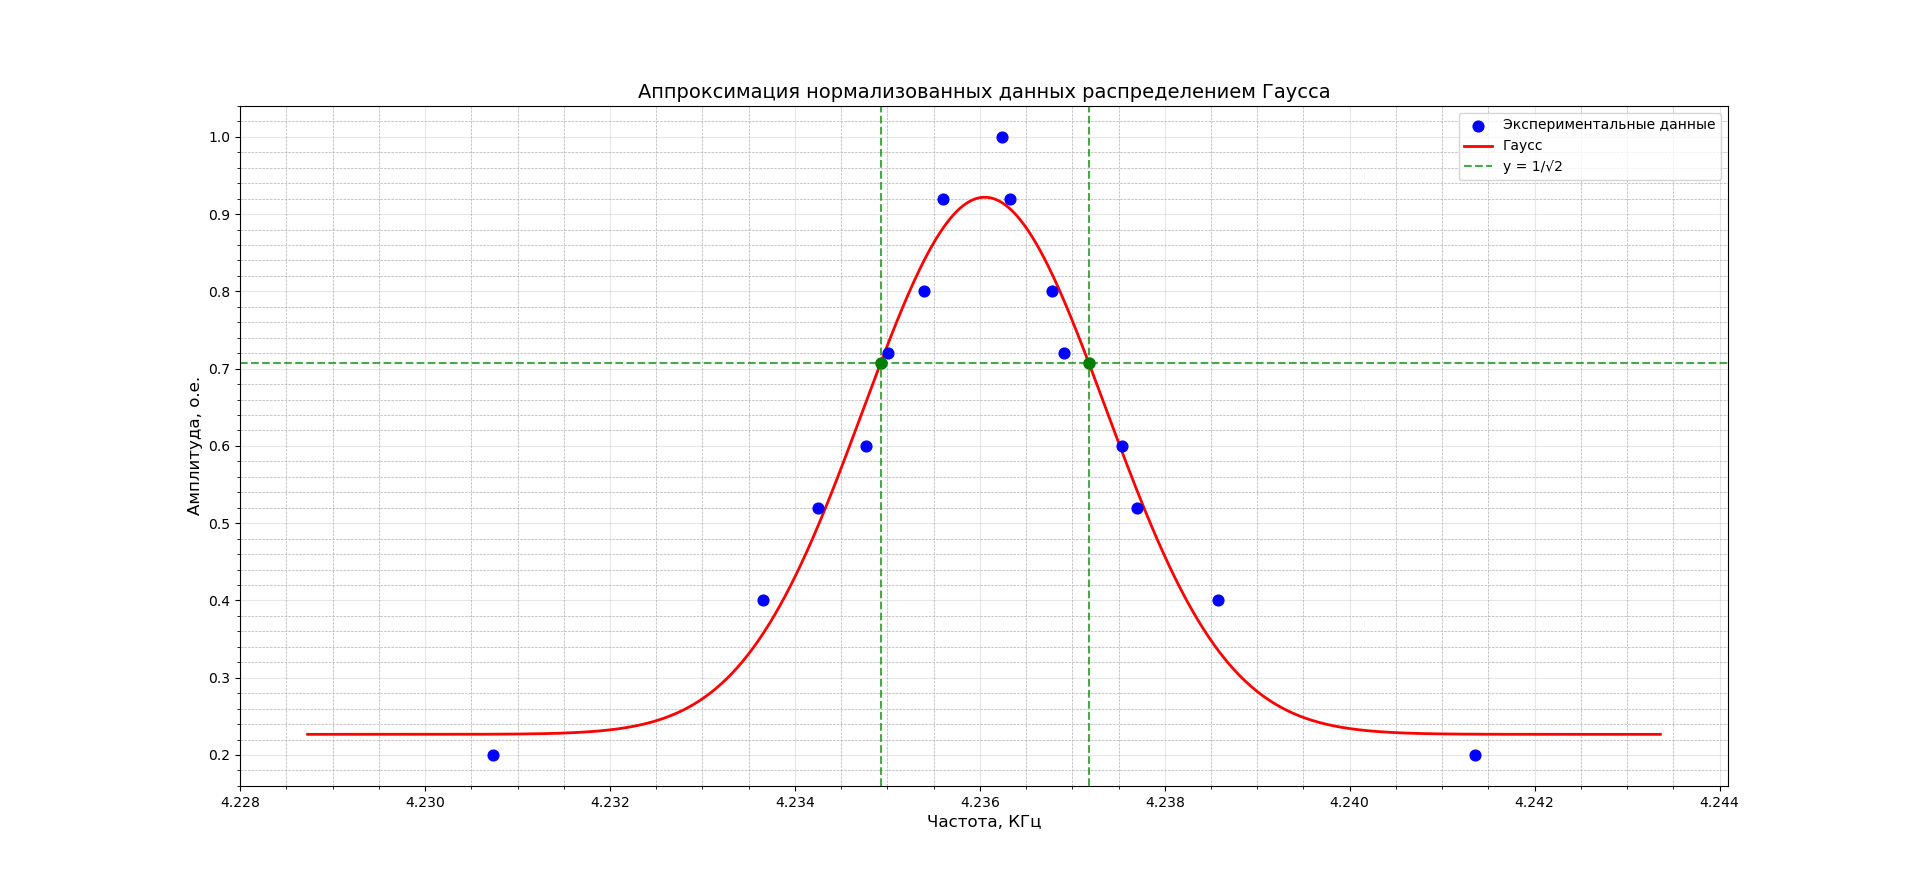
\includegraphics[width=1\linewidth]{Figure_2.png}
	\caption{Приложение 1} 
	\label{fig:mpr}
\end{figure}
\begin{figure}[h]
	\centering
	
\includegraphics[width=1\linewidth]{Figure_1.png}
	\caption{Приложение 2} 
	\label{fig:mpr}
\end{figure}
\begin{figure}[h]
	\centering
	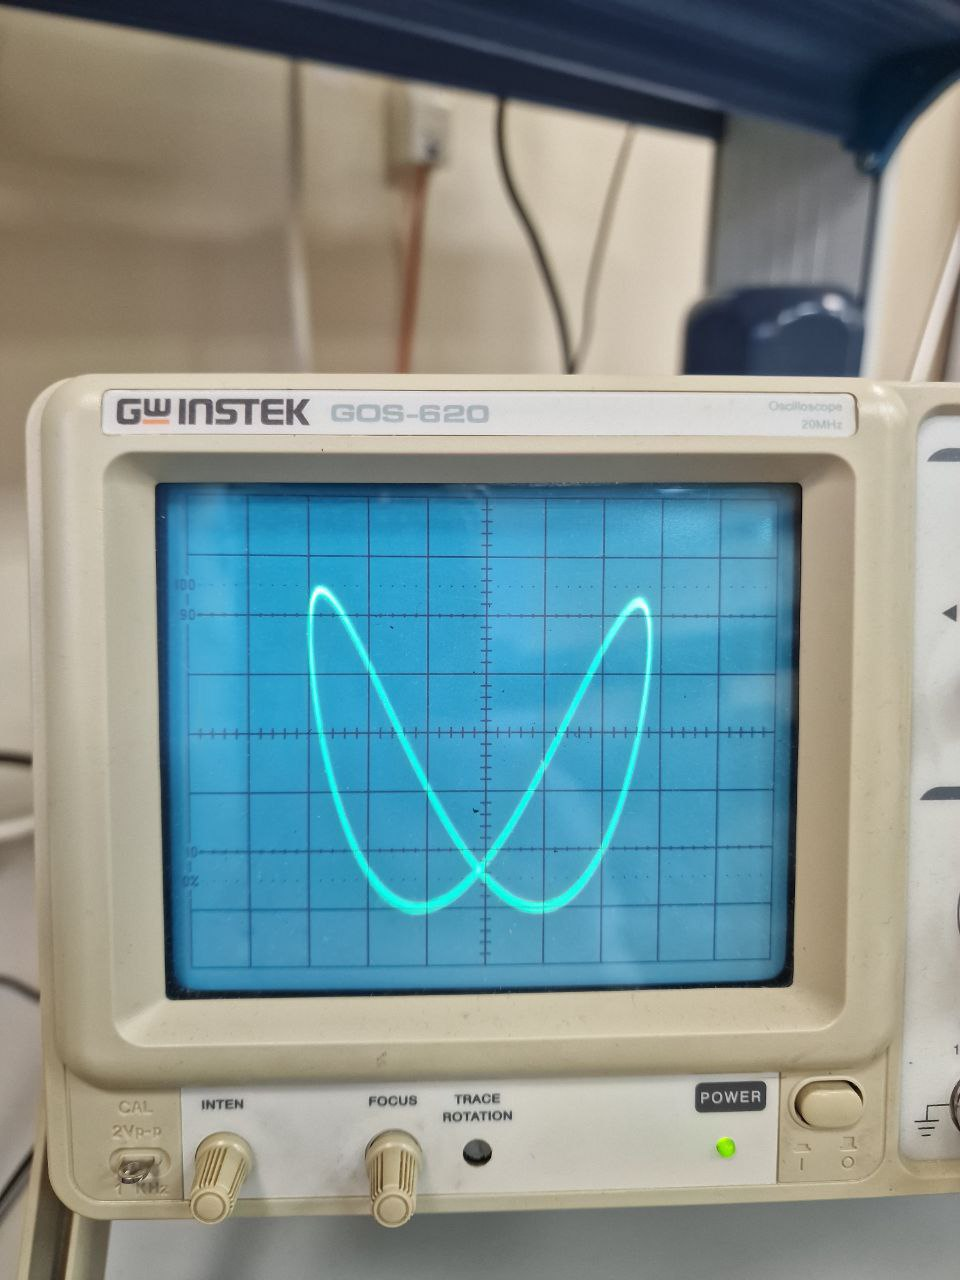
\includegraphics[width=0.5\linewidth]{lissaju.jpg}
	\caption{Приложение 3} 
	\label{fig:mpr}
\end{figure}
\end{document}

